\newpage
\begin{song}{title={Pieśń wielorybników}, interpret={EKT Gdynia}, music={tradycyjna (Bonnie Ship the Diamond)}}
\begin{multicols}{2}
    \begin{intro}
        a a a d \\
        a e a a $\times 2$
    \end{intro}
    \begin{verse}
        Nasz D^{a}iament\footnotemark{} prawie g^{e}otów już \\
        W cieśn^{a}inach nie ma kr^{e}y \\
        Na k^{a}ei piękne pa^{e}nny stoją \\
        W o^{d}czach bły^{e}szczą ł^{a}zy \smallskip \\
        Kapitan w niebo wlepia wzrok \\
        Ruszamy lada dzień \\
        Płyniemy tam, gdzie słońca blask \\
        Nie mąci nocy cień
    \end{verse}
    \begin{chorus}
        A więc krz^{a}ycz: \say{^*{e}O-- ^{a}ho!} \\
        Od^{a}wagę w ^{e}sercu mi^{a}ej \\
        Wielo^{a}rybów ^{e}cielska ^{C}groźne ^{G}są \\
        Lecz ^*{F}dosta ^{e}niemy ^{a}je $\times 2$
    \end{chorus}
    \begin{chorus*}
        a a a d \\
        a e a a $\times 2$
    \end{chorus*}
    \vfill\null\columnbreak{}
    \begin{verse}
        Hej panno, po co łzy \\
        Nic nie zatrzyma mnie \\
        Bo prędzej w lodach kwiat zakwitnie \\
        Niż wycofam się \smallskip \\
        No nie płacz mała, wrócę tu \\
        Nasz los nie taki zły \\
        Bo da dukatów wór za tran \\
        I wielorybie kły
    \end{verse}
    \begin{chorus}
        A więc krzycz: \say{O--ho!}\ldots $\times 2$
    \end{chorus}
    \begin{verse}
        Na deku stary wąchał wiatr \\
        Lunetę w ręku miał \\
        Na łodziach co zwisały już \\
        Z harpunem każdy stał \smallskip \\
        I dmucha tu, i dmucha tam  \\
        Ogromne stado w krąg \\
        Harpuny, wiosła, liny brać \\
        I ciągaj brachu ciąg
    \end{verse}
    \begin{chorus}
        A więc krzycz: \say{O--ho!}\ldots $\times 2$
    \end{chorus}
    \begin{info}
    \end{info}
    \begin{interlude}
        \textit{(wolniej)} \\
        I dla ^*{a}wielo ry^{G}ba j^{a}uż \\
        Os^*{e}ta tn^{G}i to dzi^{a}eń \\
        Bo śmi^{a}ały harp^*{C}un n^{G}ik \\
        ^*{F}U de^{G}rza w^{a}eń
    \end{interlude}
    \begin{outro}
        a a a d \\
        a e a a
    \end{outro}
\end{multicols}
\footnotetext{statek wielorybniczy \say{Diamond}, zmiażdżony przez kry lodowe w Cieśninie Davisa w 1830 r.}
\end{song}
\fancyfoot[LO,RE]{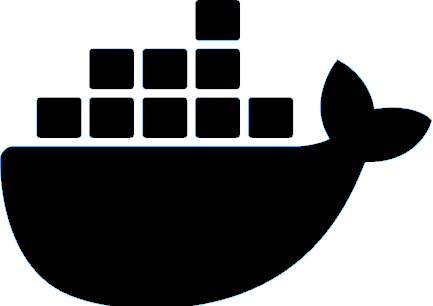
\includegraphics[height=45pt]{images/docker.png}}

